\newpage
\section{Numerical Results on Spherical Dictionaries \label{appendix:spherical}}

\Cref{fig:eta-sweep-spherical} provides experimental results identical to \Cref{fig:k-sweep} except for the use of spherical dictionaries instead of Rademacher dictionaries. Specifically, we sample codewords $F_i$ as independent vectors uniformly distributed over the unit sphere. In our experiments, coeffients are represented by half-precision floating points. \Cref{fig:eta-sweep-spherical} and \Cref{fig:eta-sweep} are almost visually identical. The small differences that exist are most visible for small values of $k.$ (Small values of $k$ correspond to ``buckets'' in the range of $\eta.$)

\begin{figure}[h]
\centering
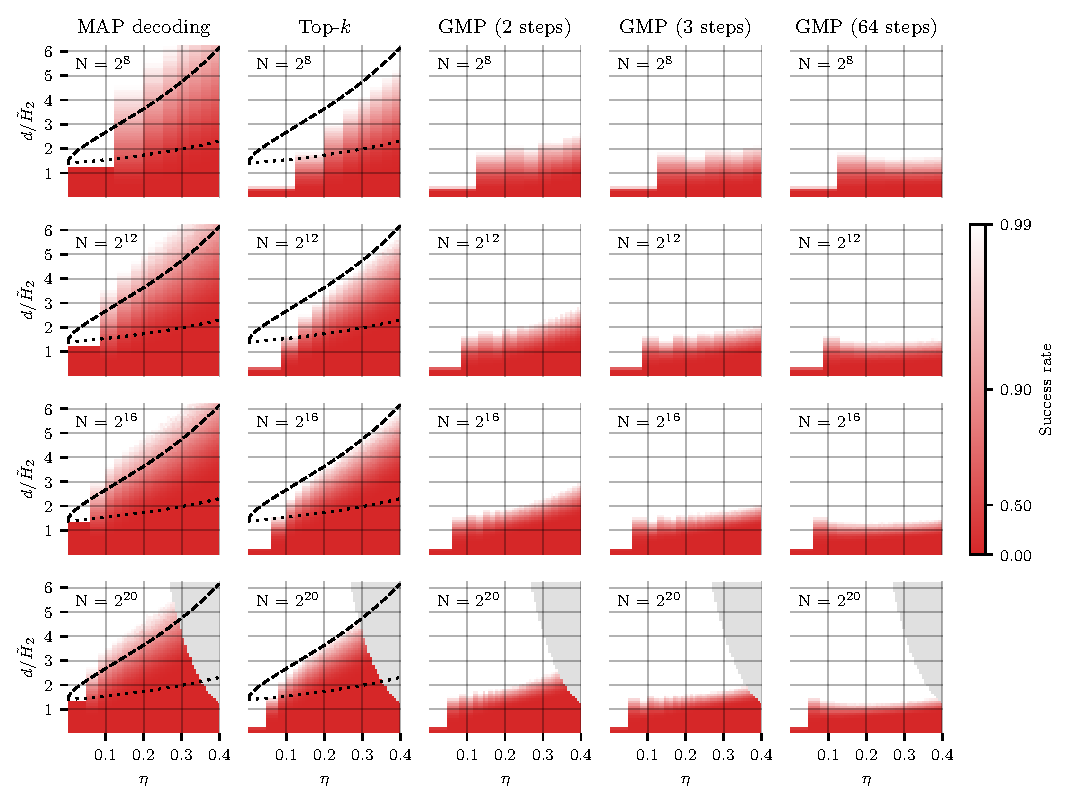
\includegraphics[width=1\textwidth]{../figures/eta_sweep_spherical}
\caption{Empirical results on spherical dictionaries, otherwise with the same experimental setup described in \Cref{sec:numerical}. Compare to \Cref{fig:k-sweep}.}
\label{fig:eta-sweep-spherical}
\end{figure}
